\newpage
\section*{CHAPTER 3. IMPLEMENTATION}
\phantomsection\label{chap:implementation}\addcontentsline{toc}{section}{CHAPTER 3. IMPLEMENTATION}
\setcounter{section}{3}
\setcounter{figure}{0}
\setcounter{subsection}{0}
\setcounter{subsubsection}{0}
\setcounter{paragraph}{0}
\setcounter{table}{0}

Chapter 3 presents the implementation of the proposed quantized HiFiC GAN accelerator. The discussion begins with the system-level architecture and hardware--software partitioning, then presents the mixed-precision quantization strategy applied to the HiFiC model and the workload analysis that identifies the residual block as the main acceleration target. It then details the internal accelerator blocks and finally describes how the design is prepared for deployment on the ZCU104 FPGA platform.

The goal of this chapter is not to redefine the HiFiC algorithm, which has already been introduced in the theoretical background, but to explain how the model is mapped into a practical hardware--software co-design. Therefore, the chapter emphasizes architectural partitioning, mixed-precision quantization, data movement, buffering, parallel computation, and the High-Level Synthesis (HLS) flow used to generate the FPGA accelerator.

%%%%%%%%%%%%%%%%%%%%%%%%%%%%%%%%%%%%%%%%%%%%%%%%%%%%%%%%%%%%%%%%%%%%%%%%%%%%%%%%%%%%%%%%%%%%%%%%%%%%
\subsection{System-Level Architecture Design}

This section describes how the design specifications introduced in Section~\ref{subsec:design_specs} of Chapter~1 -- a quantized HiFiC GAN generator accelerator on the ZCU104 platform, modeled in C/C++ and built with the Vitis HLS and Vivado tool flow -- are realized as a concrete hardware--software system.

Figure~\ref{fig:design_flow} shows the overall design flow followed in this thesis, organized into three phases: \emph{specification and analysis}, \emph{design and verification}, and \emph{synthesis and integration}.

\begin{figure}[H]
    \centering
    
\includegraphics[width=\textwidth]{Images/Design_flow.png}
    \caption{Overall design flow of the HiFiC GAN accelerator}
    \label{fig:design_flow}
\end{figure}

In the \textbf{specification and analysis} phase, the problem is defined together with the HiFiC GAN specification, followed by a state-of-the-art analysis and a system specification analysis. These steps lead to a hardware--software co-design architecture proposal that decides which parts of the inference pipeline are accelerated on the FPGA and which remain in software.

In the \textbf{design and verification} phase, the selected compute kernels are written as a C/C++ algorithm in Vitis HLS. In parallel, the pre-trained HiFiC model provides golden data for a C/C++ testbench environment. The HLS design is checked by C simulation against these golden outputs; if the results do not match, the C/C++ design is revised and the loop is repeated until functional correctness is achieved.

In the \textbf{synthesis and integration} phase, the verified design is passed through High-Level Synthesis, which produces a synthesis report and enables C/RTL co-simulation to confirm that the generated RTL behaves identically to the C model. If the design does not meet the target specifications, the C/C++ description is tuned -- through loop pipelining, array partitioning, on-chip buffering, and interface directives -- and re-synthesized. Once the targets are met, the IP core is exported and integrated into a Zynq UltraScale+ system using Vivado, where it is connected to external DDR memory and the Processing System (PS) through AXI interfaces and controlled from a Vitis software application.

\subsubsection{HiFiC GAN Model-Level Data Path}

This subsection first clarifies the model-level data path before discussing hardware partitioning. The purpose is to identify which part of the HiFiC inference pipeline should remain in software and which part should be mapped to the FPGA accelerator.

The overall HiFiC architecture used in this thesis was presented in Figure~\ref{fig:hific-architecture} of Chapter~2. The model consists of an encoder network, a hyperprior network, and a generator network. The encoder transforms the input image into a compact latent representation, while the hyperprior network provides side information for entropy modeling. The generator reconstructs the final image from the latent representation and is responsible for recovering high-quality visual details.

From the implementation perspective, the encoder and hyperprior mainly define the compression control path and model preparation flow, whereas the generator dominates reconstruction computation. As illustrated in Figure~\ref{fig:generator_structure}, the generator includes an initial convolution block, multiple residual blocks, several up-convolution blocks, and an output convolution block. The residual blocks are repeated many times and contain a large number of multiply--accumulate (MAC) operations, so they become the main candidate for FPGA acceleration. This choice is later confirmed quantitatively by the workload profiling in this chapter, which shows that the repeated residual blocks account for more than 78\% of the generator runtime.

\begin{figure}[H]
    \centering
    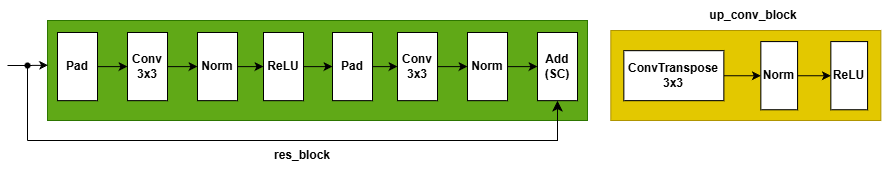
\includegraphics[width=0.9\textwidth]{Images/GAN.png}
    \caption{Generator structure with residual blocks and up-convolution blocks}
    \label{fig:generator_structure}
\end{figure}

Therefore, the system-level design decision is derived directly from the model data path: software keeps the compression front-end (encoder, hyperprior, and entropy coding), while the entire generator (decoder) is offloaded to hardware. This relationship is the basis for the hardware--software partitioning described next.

\subsubsection{System Partitioning and PS--PL Interfaces}

Based on the model-level analysis in the previous subsection, the proposed implementation follows a hardware--software co-design strategy. Tasks that require flexibility, irregular control, file handling, or model orchestration -- namely the encoder, hyperprior, and entropy coding of the compression front-end -- are executed on the Processing System (PS). The entire generator (decoder), which dominates the reconstruction computation, is offloaded to the Programmable Logic (PL) as a single accelerator IP, where parallel datapaths and streaming buffers are customized for the convolution-heavy workload.

Figure~\ref{fig:hw_sw_overview} summarizes this partitioning. The PS manages model control, parameter preparation, memory allocation, and accelerator invocation. The PL executes the generator accelerator as a single reusable compute IP. Large tensors are exchanged through shared DDR memory, while lightweight control signals are transferred through memory-mapped AXI registers.

\begin{figure}[H]
    \centering
    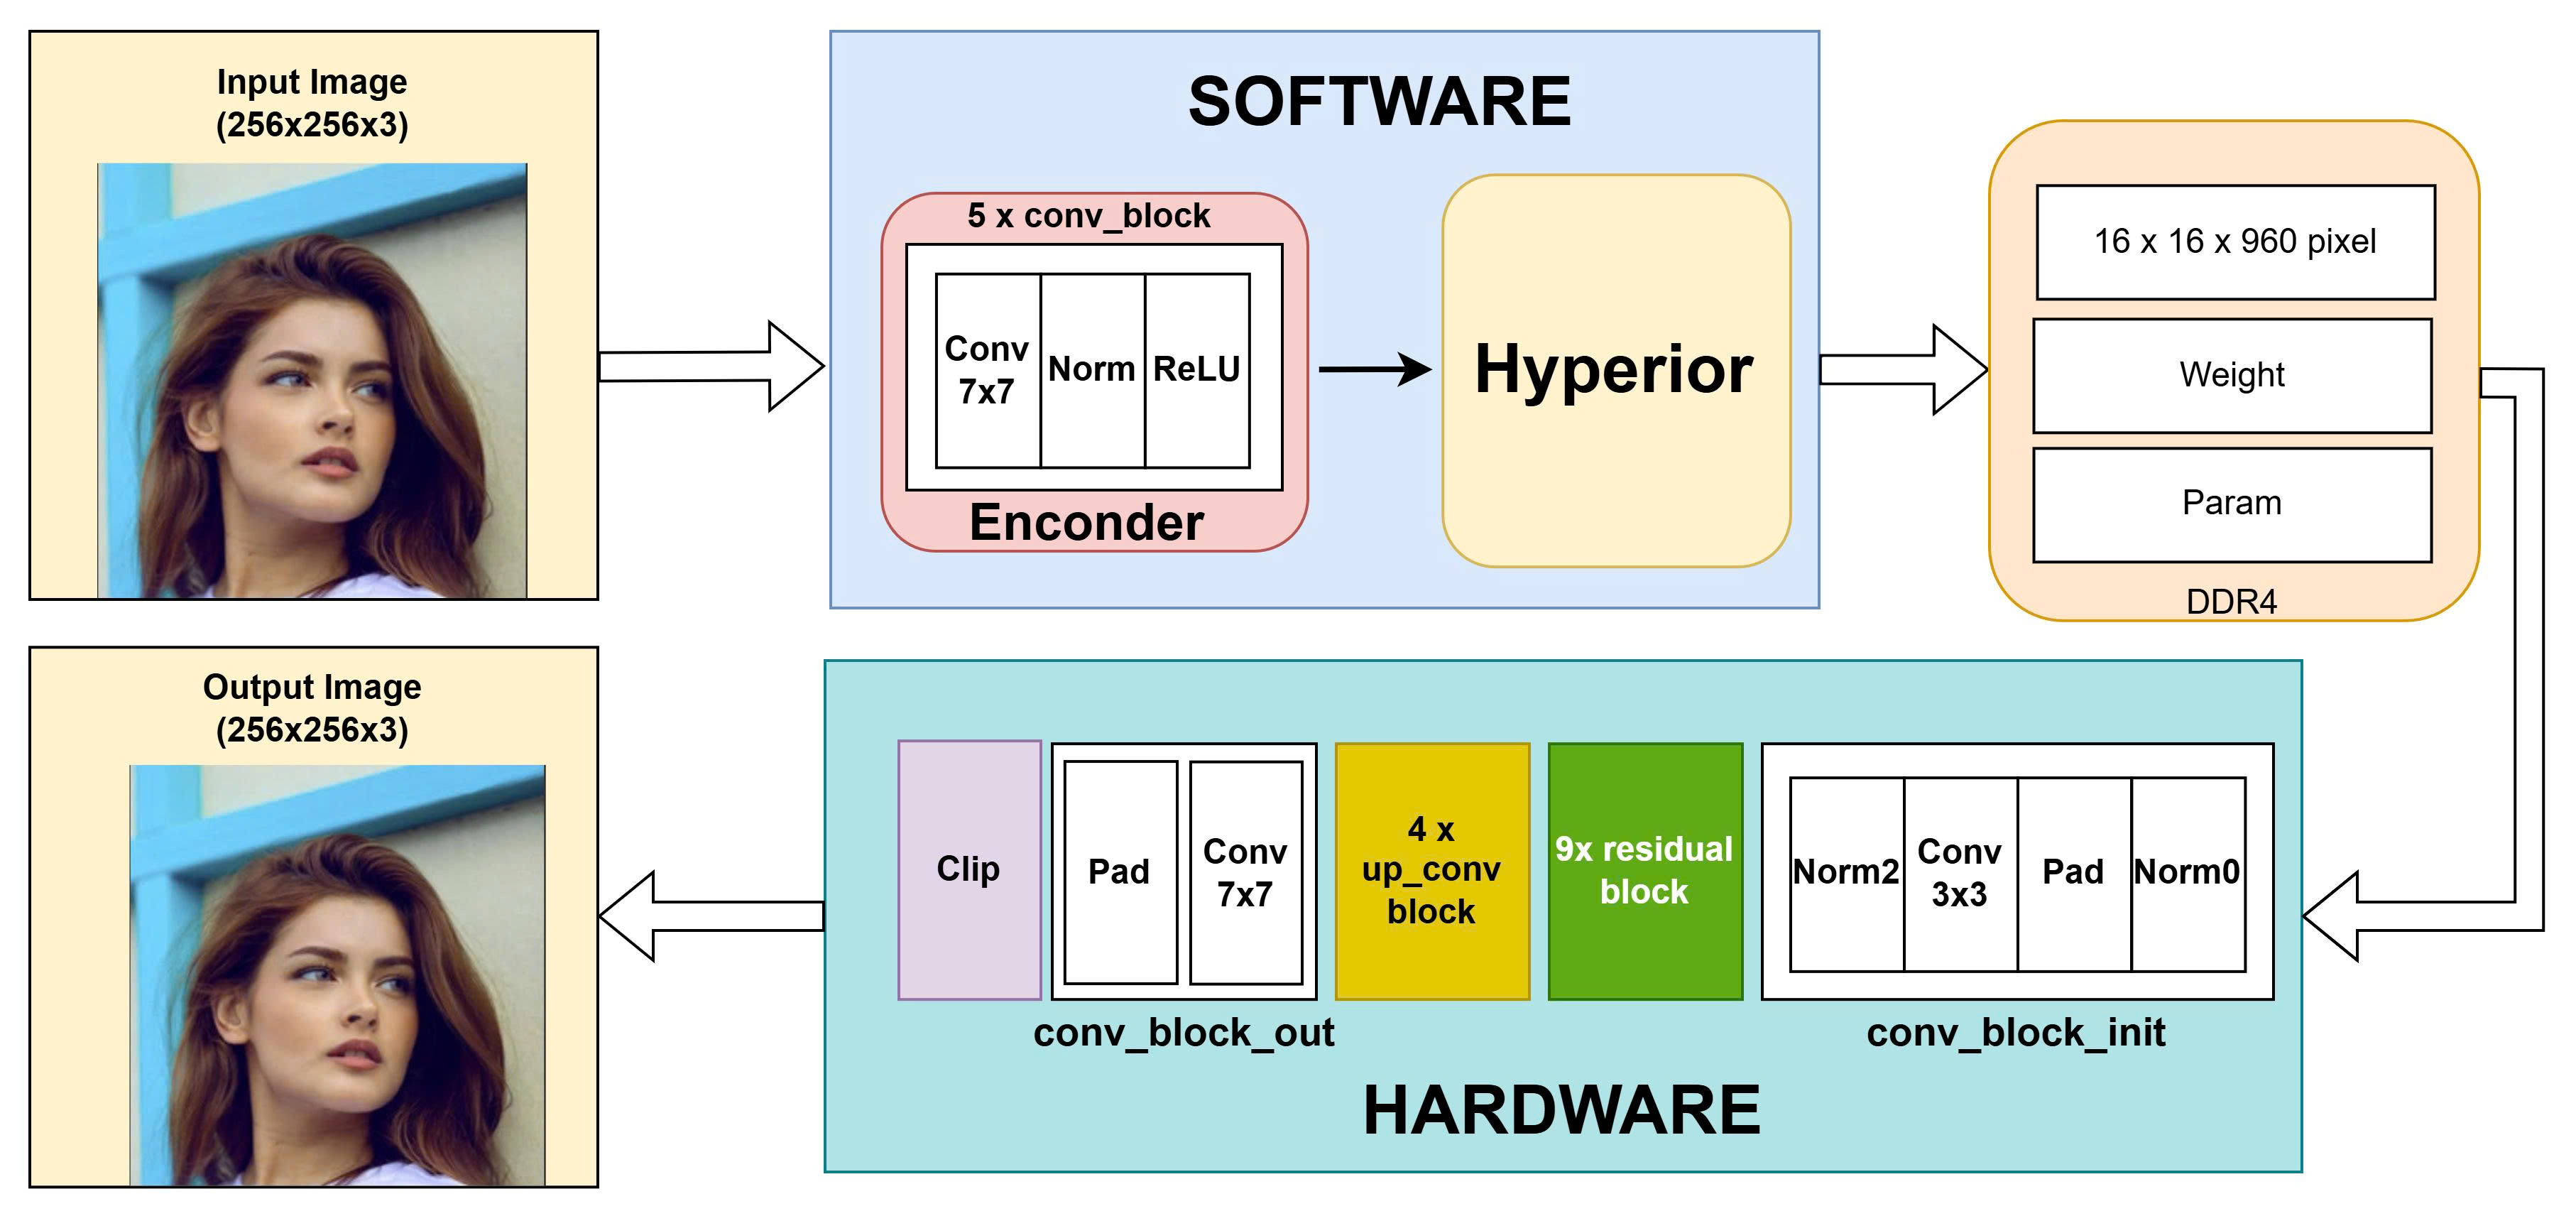
\includegraphics[width=1.0\textwidth]{Images/HW_SW.jpg}
    \caption{System-level hardware--software co-design overview of the HiFiC inference pipeline}
    \label{fig:hw_sw_overview}
\end{figure}

The PS--PL communication is organized through a small number of well-defined interfaces, as summarized in Table~\ref{tab:system_interfaces}. This interface view makes the system partition explicit and connects the high-level architecture in Figure~\ref{fig:hw_sw_overview} with the detailed generator accelerator design presented later in this chapter.

\begin{table}[H]
\centering
\caption{System-level interfaces used by the generator accelerator}
\label{tab:system_interfaces}
\begin{tabularx}{\textwidth}{|>{\raggedright\arraybackslash}p{0.24\textwidth}|>{\raggedright\arraybackslash}p{0.24\textwidth}|X|}
\hline
\textbf{Interface} & \textbf{Direction} & \textbf{Role in the system} \\
\hline
AXI4-Lite control & PS $\rightarrow$ PL & Transfers configuration values such as tensor dimensions, base addresses, start command, and status polling. \\
\hline
AXI master read & DDR $\rightarrow$ PL & Loads input feature maps, convolution weights, bias values, and normalization parameters from shared memory. \\
\hline
AXI master write & PL $\rightarrow$ DDR & Writes the reconstructed output feature maps of the generator back to shared memory. \\
\hline
Shared DDR buffers & PS $\leftrightarrow$ PL & Provide the common storage space used to exchange large tensors between software execution and hardware acceleration. \\
\hline
\end{tabularx}
\end{table}

From the software perspective, the accelerator call behaves as a coarse-grained operation. The PS prepares the input and parameter buffers in DDR, writes the required configuration values through AXI4-Lite, starts the accelerator, waits for completion, and then reads back the reconstructed image. From the hardware perspective, the PL implements the complete generator datapath with memory-mapped input and output ports, reusing the same MAC engines across the residual blocks and the other generator stages.

%%%%%%%%%%%%%%%%%%%%%%%%%%%%%%%%%%%%%%%%%%%%%%%%%%%%%%%%%%%%%%%%%%%%%%%%%%%%%%%%%%%%%%%%%%%%%%%%%%%%
\subsection{Mixed-Precision Quantization of HiFiC Model}

The deployment of learned image compression models such as HiFiC on FPGA platforms introduces significant challenges related to memory bandwidth, storage capacity, and computational efficiency. To address these constraints, a mixed-precision quantization strategy is adopted, aiming to reduce numerical precision while preserving compression performance and perceptual quality.

Figure~\ref{fig:quantize_arch_final_clean} illustrates the proposed quantization architecture applied to the HiFiC model. The quantization process is designed to operate in a post-training manner, eliminating the need for retraining and enabling rapid deployment on the target hardware.

\begin{figure}[H]
\centering
\begin{tikzpicture}[
    node distance=0.9cm and 2.6cm,
    every node/.style={font=\small},
    block/.style={
        rectangle,
        draw,
        rounded corners,
        align=center,
        minimum width=3.0cm,
        minimum height=0.85cm
    },
    smallblock/.style={
        rectangle,
        draw,
        rounded corners,
        align=center,
        minimum width=2.7cm,
        minimum height=0.75cm
    },
    arrow/.style={->, thick}
]

% ================= Left control path =================
\node[smallblock] (const) {ConstantOfShape};
\node[smallblock, below=of const] (concat) {Concat};
\node[smallblock, below=of concat] (reshape1) {Reshape};
\node[smallblock, below=of reshape1] (slice) {Slice};
\node[smallblock, below=of slice] (transpose) {Transpose};
\node[smallblock, below=of transpose] (reshape2) {Reshape};
\node[smallblock, below=of reshape2] (castL) {Cast to FP16};

% ================= Right data path =================
\node[block, right=of slice, xshift=2.4cm] (input) {Input Tensor\\FP32};
\node[smallblock, below=of input] (castR) {Cast to FP16};

% ================= Pad + Conv =================
\node[block, below=1.8cm of castR] (pad) {Pad};
\node[block, below=of pad] (conv) {Convolution Layer\\FP16};

% ================= Outputs =================
\node[smallblock, below left=1.2cm and 1.6cm of conv] (mean) {ReduceMean};
\node[smallblock, below right=1.2cm and 1.6cm of conv] (sub) {Sub};

% ================= Straight vertical arrows =================
\draw[arrow] (const) -- (concat);
\draw[arrow] (concat) -- (reshape1);
\draw[arrow] (reshape1) -- (slice);
\draw[arrow] (slice) -- (transpose);
\draw[arrow] (transpose) -- (reshape2);
\draw[arrow] (reshape2) -- (castL);

\draw[arrow] (input) -- (castR);

% ================= HARD ROUTED ORTHOGONAL MERGE =================

% Left Cast -> Pad (horizontal then vertical)
\coordinate (Lmid) at ($(castL.east)+(1.2,0)$);
\draw[arrow] (castL.east) -- (Lmid) |- (pad.west);

% Right Cast -> Pad (vertical straight)
\draw[arrow] (castR.south) -- (pad.north);

% ================= Downstream =================
\draw[arrow] (pad) -- (conv);

\coordinate (Cmid) at ($(conv.south)+(0,-0.7)$);
\draw[arrow] (conv.south) -- (Cmid) -| (mean.north);
\draw[arrow] (conv.south) -- (Cmid) -| (sub.north);

\end{tikzpicture}
\caption{Mixed-precision quantization architecture applied to convolutional layers}
\label{fig:quantize_arch_final_clean}
\end{figure}




\subsubsection{Quantization Strategy}

A post-training mixed-precision quantization approach is employed, where the internal computation of the neural network is performed using 16-bit floating-point (FP16) precision, while maintaining 32-bit floating-point (FP32) precision at the input and output interfaces. This strategy balances computational efficiency with numerical stability and compatibility with existing preprocessing and postprocessing pipelines.

The quantization strategy consists of the following key principles:
\begin{itemize}
    \item \textbf{Interface Preservation:} The input and output tensors of the HiFiC model remain in FP32 format to ensure compatibility with external modules.
    \item \textbf{Internal Precision Reduction:} All intermediate feature maps and arithmetic operations within the network are executed in FP16 precision.
    \item \textbf{Static Weight Casting:} Convolutional kernels, bias terms, and learned parameters are statically converted from FP32 to FP16 to reduce memory footprint.
\end{itemize}

To enforce this precision boundary, explicit casting operations are inserted immediately after the input layer (FP32 to FP16) and before the output layer (FP16 to FP32). Redundant casting operators introduced during automatic model conversion are identified and removed to maintain a continuous FP16 dataflow throughout the network.

\subsubsection{Operator-Level Precision Mapping}

Following quantization, the HiFiC model executes the majority of its operations within the FP16 domain. These operations can be categorized into two main groups:

\begin{itemize}
    \item \textbf{Computational Operations:} Convolution (Conv), transposed convolution (ConvTranspose), and matrix multiplication layers dominate the arithmetic workload of the Generator and are executed entirely in FP16 precision. This enables efficient utilization of FPGA DSP resources for multiply-accumulate (MAC) operations.
    \item \textbf{Non-linear and Element-wise Operations:} Activation functions (ReLU), element-wise addition, subtraction, multiplication, division, and exponential functions are also performed in FP16 precision, ensuring consistency across the computation graph.
\end{itemize}

By enforcing FP16 computation across all internal operators, the model achieves a significant reduction in memory bandwidth consumption and computational complexity, while preserving the structural integrity of the HiFiC architecture.

\subsubsection{Quantization Rationale}

The choice of FP16 precision is motivated by its favorable trade-off between numerical range and hardware efficiency. Compared to integer-based quantization schemes, FP16 offers higher dynamic range and improved stability for GAN-based architectures, where small numerical perturbations can otherwise lead to visible degradation in reconstructed images.

This mixed-precision quantization framework establishes a robust foundation for hardware acceleration of the HiFiC model on FPGA platforms, enabling efficient execution without compromising compression fidelity or perceptual quality.

%%%%%%%%%%%%%%%%%%%%%%%%%%%%%%%%%%%%%%%%%%%%%%%%%%%%%%%%%%%%%%%%%%%%%%%%%%%%%%%%%%%%%%%%%%%%%%%%%%%%
\subsection{Workload Analysis and Acceleration Target}

To determine the most suitable hardware acceleration target, the generator network was profiled on a CPU platform. The execution time of each generator block was measured on an Intel Core i9 processor operating at 2.2\,GHz. The results are summarized in Table~\ref{tab:runtime_breakdown}.

\begin{table}[H]
\centering
\caption{Runtime breakdown of HiFiC generator blocks executed on Intel Core i9 CPU @ 2.2\,GHz}
\label{tab:runtime_breakdown}
\begin{tabular}{|l|c|c|}
\hline
\textbf{Block Name} & \textbf{Execution Time (s)} & \textbf{Percentage (\%)} \\ \hline
conv\_block\_init & 23.139 & 2.16 \\ \hline
res\_block\_0 & 111.327 & 10.37 \\ \hline
res\_block\_1 & 102.859 & 9.58 \\ \hline
res\_block\_2 & 97.376 & 9.07 \\ \hline
res\_block\_3 & 96.871 & 9.03 \\ \hline
res\_block\_4 & 96.799 & 9.02 \\ \hline
res\_block\_5 & 102.545 & 9.55 \\ \hline
res\_block\_6 & 106.396 & 9.91 \\ \hline
res\_block\_7 & 113.640 & 10.59 \\ \hline
res\_block\_8 & 118.866 & 11.08 \\ \hline
upconv\_blocks (Total 1--4) & 87.696 & 8.17 \\ \hline
conv\_block\_out & 15.588 & 1.45 \\ \hline
Others (Add, Overhead) & 0.088 & 0.03 \\ \hline
\textbf{Total Runtime} & \textbf{1073.19} & \textbf{100} \\ \hline
\end{tabular}
\end{table}

The profiling result shows that the residual blocks dominate the generator runtime. Together, the repeated ResBlocks account for more than 78\% of the total execution time, while the initial convolution, up-convolution blocks, and output convolution occupy a much smaller share. This makes the ResBlock the most effective target for acceleration.

The ResBlocks are also attractive from a hardware design perspective because they share a regular computation pattern. Each block is mainly composed of convolution, normalization, activation, and residual addition. The convolution layers reuse the same local-window structure across many spatial positions and channels, which matches the strengths of FPGA architectures: local buffering, parallel MAC units, and pipelined execution.

Although the residual blocks dominate the runtime, the proposed accelerator implements the \emph{complete} generator on hardware, so that the entire reconstruction path runs on the FPGA without returning intermediate feature maps to software. The compression front-end (encoder, hyperprior, and entropy coding) remains in software. This scope keeps the heaviest computation -- the residual blocks -- on dedicated hardware while still producing the final image entirely within the Programmable Logic.

%%%%%%%%%%%%%%%%%%%%%%%%%%%%%%%%%%%%%%%%%%%%%%%%%%%%%%%%%%%%%%%%%%%%%%%%%%%%%%%%%%%%%%%%%%%%%%%%%%%%
\subsection{Detailed Internal Block Design}

This section describes the internal architecture of the proposed accelerator. The entire HiFiC generator is implemented as a single HLS IP, \texttt{full\_generator\_top}, organized into three main cores: the \textbf{Fusion Core} (executes the initial convolution block, nine residual blocks, and the global skip addition), the \textbf{UpConv Block Core} (executes four transposed-convolution up-sampling blocks), and the \textbf{Conv77 Core} (executes the final $7\times7$ convolution that produces the RGB image). Packing the whole generator into one IP allows the multiply--accumulate (MAC) engines to be reused across cores and simplifies system integration, at the cost of a tight on-chip resource budget. The explanation below begins with the overall accelerator architecture, then describes the common building blocks (data buffering and processing elements), and finally details the implementation of each core.

\subsubsection{Overall Generator Accelerator Architecture}

At the top level, the generator accelerator is organized into three cores, as shown in Figure~\ref{fig:gan_accelerator_concept}: the \textbf{Fusion Core}, the \textbf{UpConv Block Core}, and the \textbf{Conv77 Core}. Each core is an independent hardware module that communicates with external DDR memory through its own pair of AXI4 master interfaces -- one for reading input feature maps, weights, and parameters, and one for writing the resulting output feature maps. The cores are invoked sequentially under software control to realize the complete generator datapath. Internally, every core reuses the same convolution-then-normalization-and-activation motif, which is why a small number of hardware engines can implement the whole generator network. Because the Fusion Core is the largest and most representative of this pattern, its internal datapath is described in detail first, and the lighter UpConv Block and Conv77 cores are then presented as variations of it.

\begin{figure}[H]
    \centering
    
\includegraphics[width=0.9\textwidth]{Images/GAN_accelarator.png}
    \caption{Overall architecture of the HiFiC GAN accelerator showing the three main cores (Fusion Core, UpConv Block Core, Conv77 Core) connected via AXI4 master interfaces}
    \label{fig:gan_accelerator_concept}
\end{figure}

\subsubsection{Fusion Core}

The Fusion Core executes the initial convolution block (CBI), the nine residual blocks, and the global skip addition. Its computational pattern is the residual block shown in Figure~\ref{fig:resblock_flow}: two $3\times3$ convolutions, each followed by normalization, with a ReLU between them and a skip connection that adds the block input to its output. The remainder of this subsection presents the core bottom-up: first the data-feeding building blocks (line buffer, window, and boundary handling), then the processing element that performs the arithmetic, then how these are assembled into a two-pass convolution-and-normalization datapath, and finally the complete Fusion Core block diagram.

\begin{figure}[H]
    \centering
    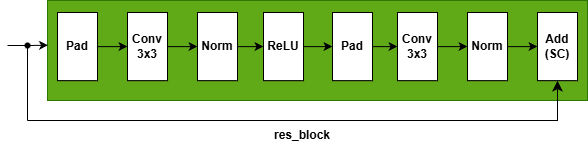
\includegraphics[width=1.0\textwidth]{Images/resblock.png}
    \caption{Computational flow of a residual block in the HiFiC generator}
    \label{fig:resblock_flow}
\end{figure}

\subsubsection*{Line Buffer, Window, and Boundary Handling}

The convolution engine processes convolution windows in a streaming manner. Instead of repeatedly loading the same pixels or feature values from external memory, the design stores recently used rows in on-chip line buffers. For a $3 \times 3$ convolution, two previous rows are sufficient because the current row is provided by the input stream.

\begin{figure}[H]
    \centering
    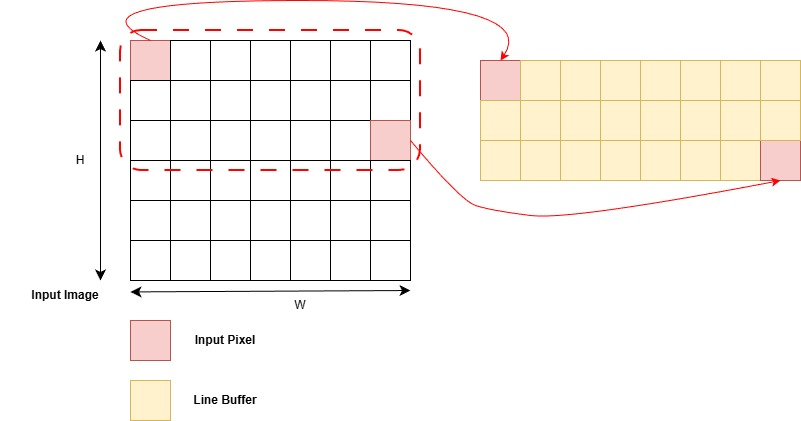
\includegraphics[width=0.8\textwidth]{Images/Line Buffer.jpg}
    \caption{Two-line buffer structure for streaming convolution}
    \label{fig:line_buffer_structure}
\end{figure}

Figure~\ref{fig:line_buffer_structure} illustrates the two-line buffer organization. As new feature values arrive in raster-scan order, the buffer keeps the spatial relationship between adjacent rows. This allows the accelerator to construct valid convolution windows without reloading the same rows from DDR memory.

\begin{figure}[H]
    \centering
    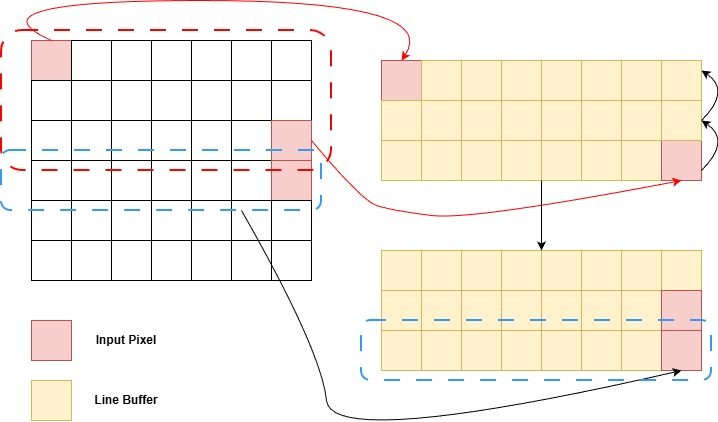
\includegraphics[width=0.8\textwidth]{Images/Line buffer flow.jpg}
    \caption{Two-line buffer dataflow and update mechanism}
    \label{fig:line_buffer_flow}
\end{figure}

The update behavior is shown in Figure~\ref{fig:line_buffer_flow}. At each new input position, stored values are shifted to keep the previous rows aligned with the current row. This structure converts external memory traffic into local buffer reuse, which is essential for high-throughput convolution on FPGA.

\begin{figure}[H]
    \centering
    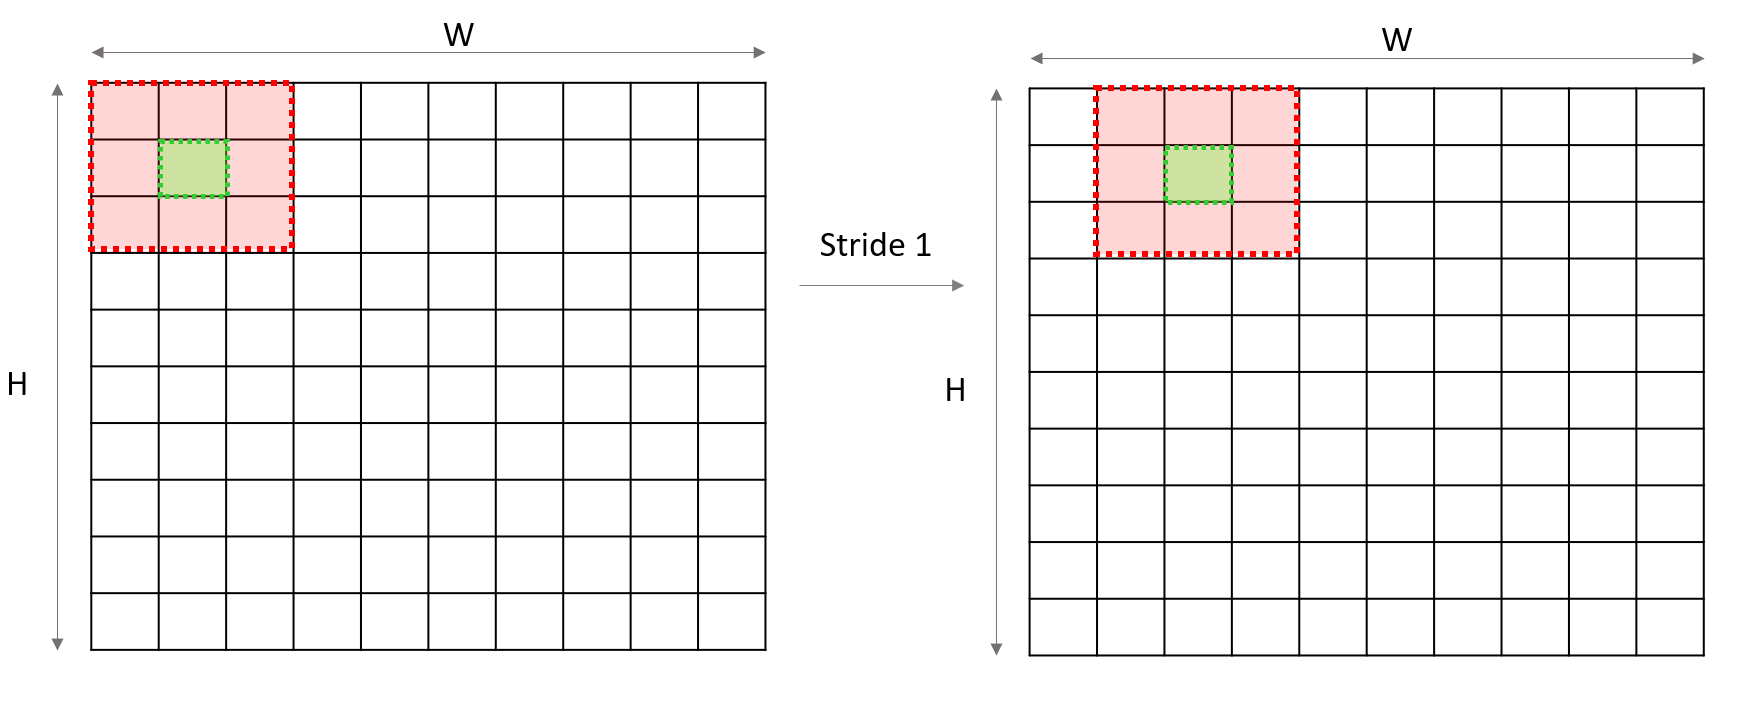
\includegraphics[width=0.6\textwidth]{Images/window.png}
    \caption{Sliding window structure for convolution processing}
    \label{fig:sliding_window}
\end{figure}

After the line buffer prepares neighboring rows, a sliding window extracts the local $3 \times 3$ region required by each convolution operation. The window structure in Figure~\ref{fig:sliding_window} provides the input values for the PE cluster. In the proposed design, multiple window positions on the same row can be generated in parallel so that several output pixels are computed at the same time.

\begin{figure}[H]
    \centering
    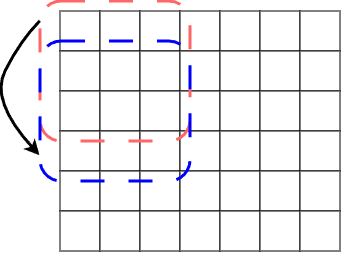
\includegraphics[width=0.6\textwidth]{Images/Window Data Update.drawio.png}
    \caption{Parallel window update mechanism with vertical-only movement}
    \label{fig:window_update}
\end{figure}

Figure~\ref{fig:window_update} shows the window update mechanism used to support parallel processing. Rather than moving a single window across the row one position at a time, the architecture assigns multiple horizontal positions to different processing lanes. The input stream then advances to the next row, while each lane maintains the correct local neighborhood for its assigned output position.

Boundary handling is implemented using reflection padding, as shown in Figure~\ref{fig:reflection_padding}. Reflection padding mirrors feature values at the border, preserving local continuity near image boundaries. This is suitable for image reconstruction workloads because it avoids the abrupt border discontinuities that may be introduced by simple zero padding.

\begin{figure}[H]
    \centering
    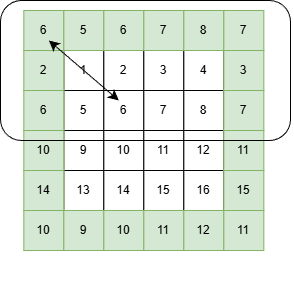
\includegraphics[width=0.6\textwidth]{Images/Reflect Pad.png}
    \caption{Reflection padding used in the generator network}
    \label{fig:reflection_padding}
\end{figure}

\subsubsection*{Processing Element Architecture}

The Processing Element (PE) is the basic arithmetic unit of the accelerator. Each PE computes one convolution result by multiplying input feature values with the corresponding kernel weights and accumulating the products.

\begin{figure}[H]
    \centering
    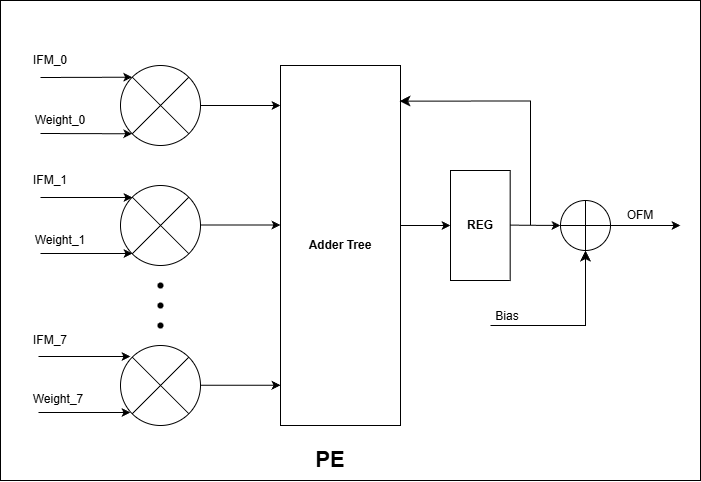
\includegraphics[width=0.7\textwidth]{Images/PE.png}
    \caption{Processing Element (PE) architecture for convolution computation}
    \label{fig:pe_architecture}
\end{figure}

As shown in Figure~\ref{fig:pe_architecture}, each PE contains eight parallel multipliers (eight MAC operations per cycle), an adder tree, an accumulation register, and bias addition. The multipliers are mapped to FPGA DSP resources, while the adder tree reduces the partial products with low latency. Multiple PEs are instantiated to form a PE cluster: the Fusion Core uses sixteen PEs ($\text{PEs}_F = 16$), giving $16 \times 8 = 128$ MAC operations per cycle when the inner MAC loop runs at $\text{II}=1$. Each PE is assigned to a different output column or lane, which increases throughput by computing several convolution outputs in parallel while reusing the same buffered input data across lanes.

A key difficulty with FP16 accumulation is that a half-precision adder has a latency of three to four cycles, which would normally prevent a new accumulation every cycle. To still reach $\text{II}=1$, the design uses a \emph{rotating accumulator}: instead of a single accumulator, each PE keeps a small array of partial sums \texttt{psum[PE][D]} and rotates the write index every cycle (for example \texttt{acc\_idx = i \& 3} for depth four). The distance between two read-after-write dependencies on the same slot then equals the accumulator depth, which is greater than or equal to the adder latency, so the pipeline never stalls. After the loop finishes, the partial sums in each slot are reduced into the final result.

\subsubsection*{Two-Pass Convolution-and-Normalization Datapath}

The line buffers and PE cluster described above are combined into two reusable functional units: a \textbf{Convolution Functional Unit (Conv FU)} that contains the MAC array (the PE cluster), and a \textbf{Normalization/Activation Functional Unit (Norm/Act FU)} that performs channel normalization and the activation function. Because each convolution layer is followed by normalization and activation, the datapath is naturally organized as two passes over the feature map: a convolution pass produced by the Conv FU, followed by a normalization-and-activation pass produced by the Norm/Act FU. Figure~\ref{fig:resblock_architecture} shows this datapath for a residual block, including input-feature buffering, weight buffering, the PE cluster, output buffering, the normalization/activation logic, and a skip-connection buffer.

\begin{figure}[H]
    \centering
    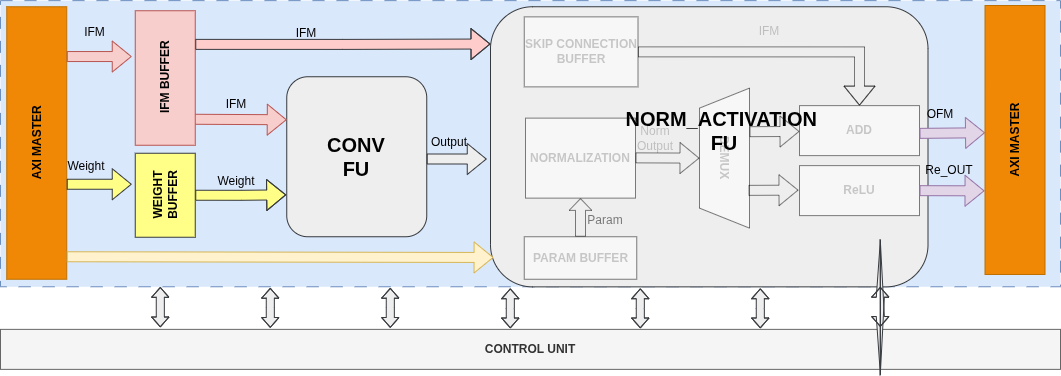
\includegraphics[width=0.9\textwidth]{Images/resblock_architecture.png}
    \caption{Convolution-then-normalization datapath of the Fusion Core, shown for a residual block}
    \label{fig:resblock_architecture}
\end{figure}

Figure~\ref{fig:two_pass_architecture} and Figure~\ref{fig:pipeline_timing} illustrate how the convolution pass and the normalization/activation pass are overlapped. While the Norm/Act FU processes one row, the Conv FU can already compute the next row, so after an initial warm-up the two passes run concurrently. This overlap, together with the rotating accumulator that keeps the MAC loop at $\text{II}=1$, is the main reason the design sustains a high MAC utilization.

\begin{figure}[H]
    \centering
    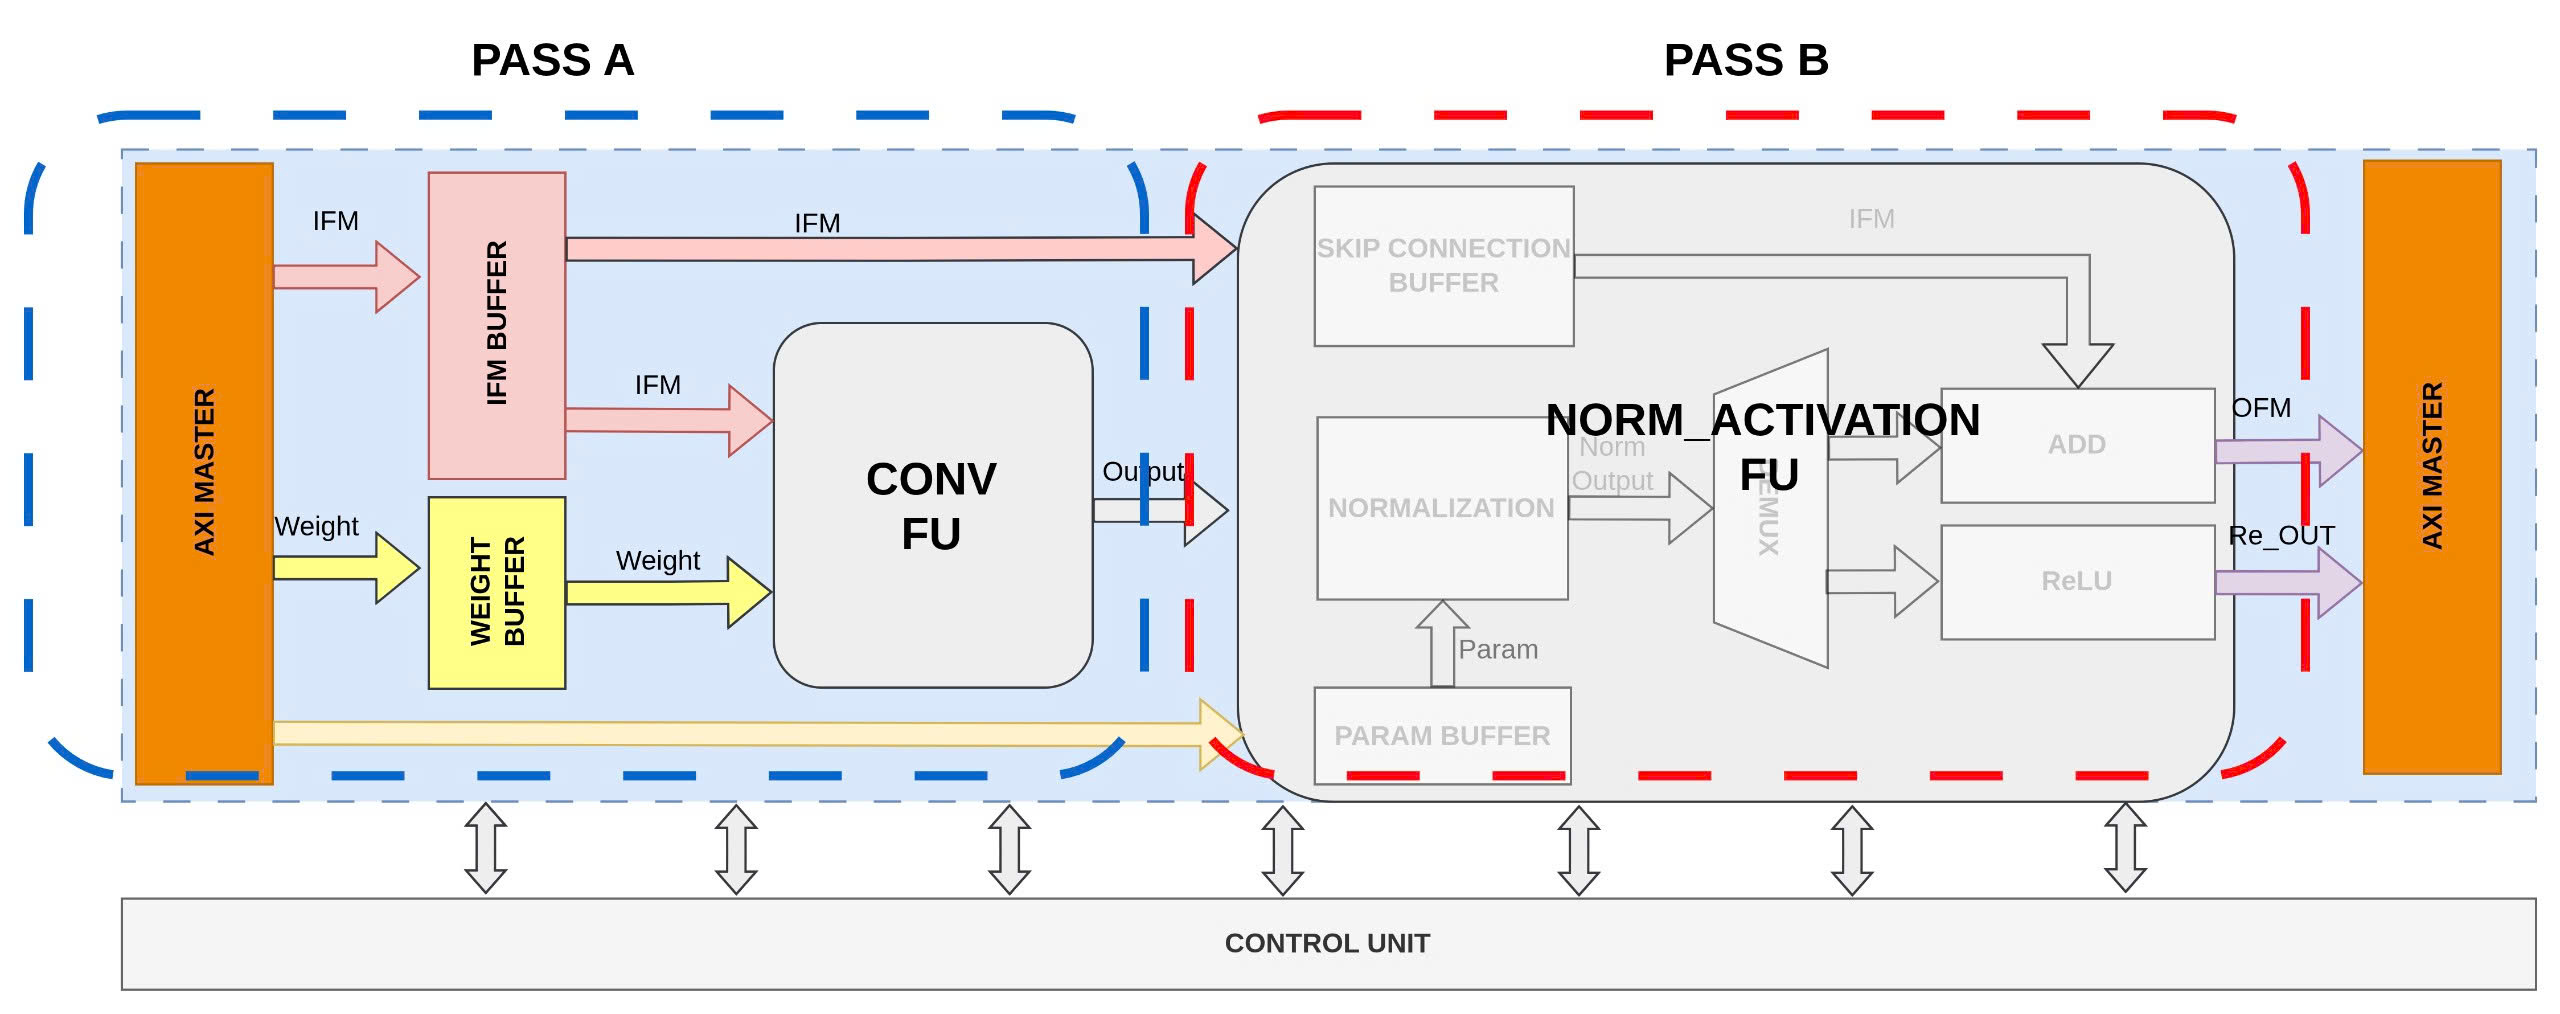
\includegraphics[width=1.0\textwidth]{Images/two_pass.jpg}
    \caption{Overlap of the convolution pass and the normalization/activation pass}
    \label{fig:two_pass_architecture}
\end{figure}

\begin{figure}[H]
    \centering
    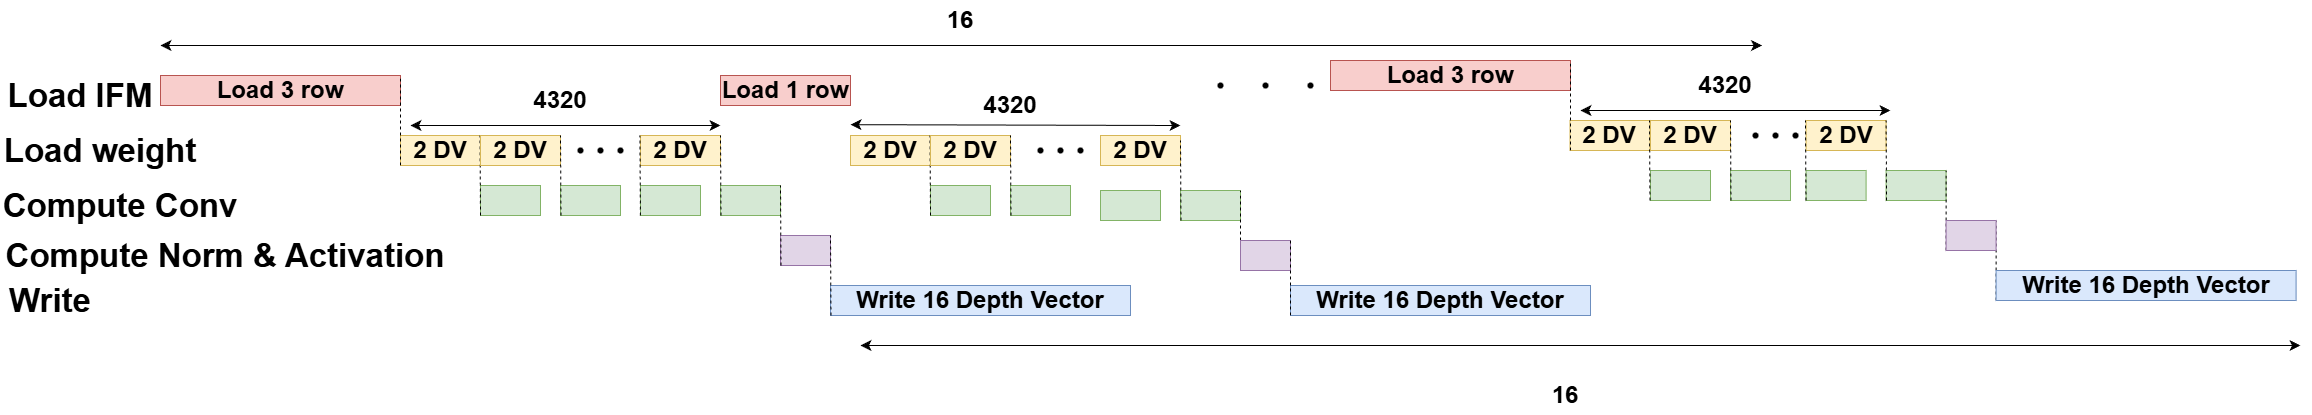
\includegraphics[width=0.95\textwidth]{Images/Pipeline Timing.png}
    \caption{Pipeline timing diagram showing overlapped loading, convolution, normalization/activation, and output writing}
    \label{fig:pipeline_timing}
\end{figure}

\subsubsection*{Fusion Core Block Diagram}

A single shared engine implements the initial convolution block, the nine residual blocks, and the global skip addition. Because the CBI, the nine residual blocks, and the global add all operate on the same $16\times16\times960$ tensor, they are mapped to one hardware instance that is invoked repeatedly with different parameters, rather than replicated. To keep this as a single instance, every call passes the same set of ports; if some calls passed null pointers and others did not, the tool would infer two different instances and exceed the on-chip memory budget. The engine uses sixteen PEs with the rotating accumulator, and stores a large skip tensor in UltraRAM (URAM): a \emph{skip-connection buffer} that holds the input of each residual block until its residual add and the CBI output until the global add. The complete block diagram, which brings together the AXI master interfaces, the input/weight/parameter buffers, the PE cluster, the normalization/activation logic, and the URAM skip buffers, is shown in Figure~\ref{fig:fusion_core}.

\begin{figure}[H]
    \centering
    
\includegraphics[width=\textwidth]{Images/FusionCore_HighLevel.png}
    \caption{Block diagram of the Fusion Core: AXI master input, normalization, ping-pong buffers, the PE cluster (PE0--PE15), normalization/activation, and the URAM skip buffers}
    \label{fig:fusion_core}
\end{figure}

\subsubsection{UpConv Block Core}

The UpConv Block Core performs the four up-sampling blocks of the generator. As shown in Figure~\ref{fig:ucb_model}, each block follows the same network pattern: a $3\times3$ transposed convolution, followed by channel normalization and a ReLU activation. Every transposed convolution uses stride two, so each block doubles the spatial resolution and halves the channel count, as summarized in Table~\ref{tab:upconv_steps}.

\begin{figure}[H]
    \centering
    
\includegraphics[width=0.65\textwidth]{Images/UCB_Model_architeture.png}
    \caption{Network pattern of an up-convolution block (UCB): a $3\times3$ transposed convolution followed by normalization and ReLU}
    \label{fig:ucb_model}
\end{figure}

\begin{table}[H]
\centering
\caption{Resolution and channel changes through the four up-convolution blocks}
\label{tab:upconv_steps}
\begin{tabular}{|c|c|c|}
\hline
\textbf{Block} & \textbf{Input} & \textbf{Output} \\
\hline
UCB\_0 & $16\times16\times960$ & $32\times32\times480$ \\
\hline
UCB\_1 & $32\times32\times480$ & $64\times64\times240$ \\
\hline
UCB\_2 & $64\times64\times240$ & $128\times128\times120$ \\
\hline
UCB\_3 & $128\times128\times120$ & $256\times256\times60$ \\
\hline
\end{tabular}
\end{table}

\subsubsection*{Computation Model: Transposed Convolution as Scatter}

Following the scatter formulation of transposed convolution introduced in Chapter~2, this core implements each up-convolution block as a \emph{scatter-and-accumulate} operation: every input pixel distributes its weighted contributions to several output positions according to the $3\times3$ kernel and the stride-two pattern. Because of the stride, the input-to-output mapping is sparse, so for any given output row only part of the kernel taps actually contribute while the rest are skipped. As in the Fusion Core, a single shared engine serves all four blocks; the input source is selected by an internal mode parameter so that the tool infers only one hardware instance.

\subsubsection*{Hardware Architecture: Differences from the Fusion Core}

At the block level, the UpConv Block Core reuses almost the same organization as the Fusion Core: the same AXI master interfaces, input/weight/parameter buffering, streaming line buffers, and the overall convolution-then-normalization datapath. The one essential difference is the Processing Element: the standard PE of the Fusion Core is replaced by a \textbf{Transpose PE}, shown in Figure~\ref{fig:transpose_pe}. The Transpose PE keeps the same multiplier array, adder tree, and bias addition, but adds two extra stages at its output -- a \textbf{Scatter} stage and an \textbf{Accumulator} stage.

\begin{figure}[H]
    \centering
    
\includegraphics[width=\textwidth]{Images/Transpose_PE.png}
    \caption{Block diagram of the Transpose PE in the UpConv Block Core}
    \label{fig:transpose_pe}
\end{figure}

To understand why these two stages are needed, it helps to contrast the two operations. In the Fusion Core, the convolution is a \emph{gather}: each output pixel collects a fixed $3\times3$ input window, so once a PE finishes its multiply-accumulate the result is already the final output value and can be written out in place. The computation is output-stationary, and a standard PE therefore needs nothing beyond its MAC and bias stages. The transposed convolution is the opposite, a \emph{scatter}: one input pixel, multiplied by the kernel, contributes to several different output positions, and conversely each output position receives contributions from several input pixels and kernel taps that are produced in different loop iterations. A Transpose PE result is thus only a \emph{partial} contribution to an output pixel, never its final value. This is precisely the gap that the Scatter and Accumulator stages close.

\textbf{Why the Scatter stage.} A normal PE always writes its result to the same, in-place output location. A Transpose PE cannot, because the upsampling pattern sends each partial result to a different, non-contiguous output position. The Scatter stage performs this routing: from the input pixel position and the active kernel tap it computes the destination address in the output feature map and steers the partial result there. For the stride-two transposed convolution used here, an input pixel at column $w_i$ contributes through kernel tap $k_w$ to output column $w_o = 2\,w_i + k_w - 1$; the Scatter stage applies this index mapping so that each partial result lands at the correct upsampled position. In short, it replaces the fixed write address of a normal PE with a computed, data-dependent one dictated by the stride.

\textbf{Why the Accumulator stage.} Because several partial results are scattered onto the \emph{same} output position at different times, that position cannot simply be overwritten -- each new contribution has to be \emph{added} to what is already there. The Accumulator stage carries out this read--modify--write: it reads the partial sum currently stored at the scattered output position, adds the new contribution, and writes the updated value back. These running sums are kept in a row-wide accumulation buffer (mapped to on-chip URAM) that persists across loop iterations until every input pixel has scattered its contribution; only at that point is an output pixel complete and ready for normalization. The Fusion Core needs neither stage, because its gather computation writes each output pixel exactly once and never has to read it back.

\subsubsection*{Execution Timing}

Figure~\ref{fig:upconv_timing} shows the timing path of the up-convolution engine, in which the loading of input rows is overlapped with the computation of output rows. The cycle counts in the figure are measured for the first up-convolution block, UCB\_0 (input $16\times16\times960$, output $32\times32\times480$): after a short initialization (\texttt{RESET\_ROW\_ACC}, $1{,}026$ cycles, and \texttt{LOAD\_PARAMS} for bias, beta, and gamma, $162$ cycles), the engine iterates the tile loop $41$ times, each iteration loading a weight tile ($4{,}449$ cycles) and performing the 8-channel MAC compute ($69{,}483$ cycles). The tile loop therefore dominates at $41 \times 69{,}483 = 2{,}848{,}803$ cycles, followed by the normalization-and-write stage (statistics and normalization, $23{,}363$ cycles), giving a total latency of $2{,}878{,}197$ cycles for UCB\_0.

\begin{figure}[H]
    \centering
    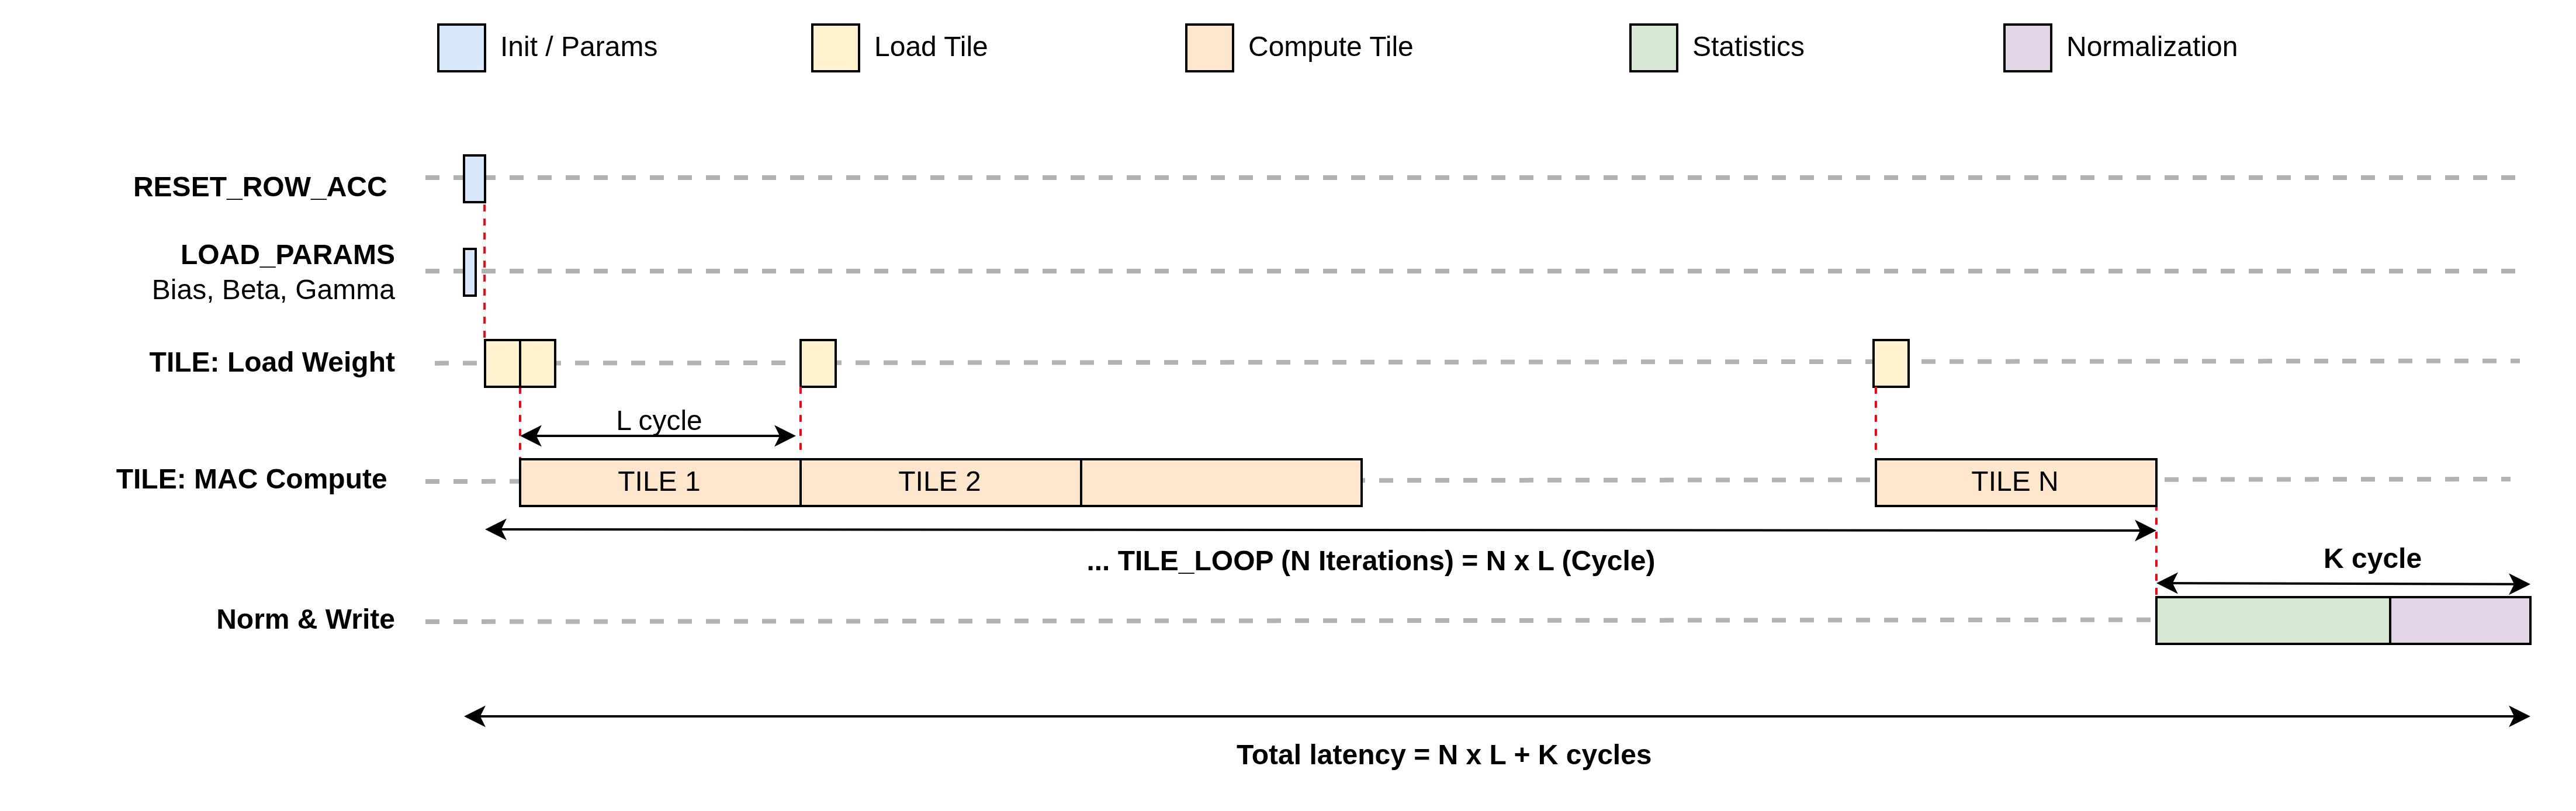
\includegraphics[width=\textwidth]{Images/timing_UCB.jpg}
    \caption{Timing path of the up-convolution engine for the first up-convolution block (UCB\_0), overlapping input-row loading with output-row computation. All cycle counts shown are measured for UCB\_0.}
    \label{fig:upconv_timing}
\end{figure}

\subsubsection{Conv77 Core}

The Conv77 Core implements the final output block: reflection padding, a $7\times7$ convolution that maps the 60 feature channels to the 3 RGB channels, and a clipping operation. Its Processing Element reuses the same architecture as the Fusion Core PE -- the same multiplier array, accumulation, and bias addition -- and differs only in the adder tree. Because the kernel is $7\times7$ instead of $3\times3$, each output value is the sum of a larger number of partial products, so the adder tree is widened and deepened accordingly to reduce them. Unlike the other two cores, the Conv77 Core uses only Block RAM (no URAM) for its small input-window and weight buffers. A final clipping to the range $[0,1]$ is applied, as required by the HiFiC specification for normalized images.

\subsubsection{On-Chip Memory Layout}

Table~\ref{tab:onchip_buffers} summarizes the main on-chip buffers. Large, persistent skip tensors and the up-convolution row accumulator are placed in URAM, while sliding-window buffers that require many parallel access ports are placed in Block RAM. For example, the Fusion input-window buffer is partitioned for sixteen parallel lanes; if it were placed in URAM it would require more blocks than the device provides, so it is mapped to BRAM instead.

\begin{table}[H]
\centering
\caption{Main on-chip buffers of the generator accelerator}
\label{tab:onchip_buffers}
\begin{tabularx}{\textwidth}{|>{\raggedright\arraybackslash}p{0.24\textwidth}|>{\raggedright\arraybackslash}p{0.20\textwidth}|>{\raggedright\arraybackslash}p{0.12\textwidth}|X|}
\hline
\textbf{Buffer} & \textbf{Size} & \textbf{Type} & \textbf{Purpose} \\
\hline
Skip-connection buffer & $16\times16\times960$ & URAM & residual skip of each res\_block \\
\hline
Global skip buffer & $16\times16\times960$ & URAM & CBI output for the global add \\
\hline
Row accumulator & $256\times480$ & URAM (32 banks) & up-convolution output accumulation \\
\hline
Fusion window buffer & $4\times W\times60$ & BRAM & sliding-window input feature map \\
\hline
Conv77 window buffer & $7\times14\times64$ & BRAM & sliding window of the $7\times7$ convolution \\
\hline
Conv77 weight buffer & $3\times7\times7\times64$ & BRAM & on-chip $7\times7$ weights \\
\hline
\end{tabularx}
\end{table}

\subsubsection{Top-Level Kernel Interface}

The HLS kernel \texttt{full\_generator\_top} exposes a memory-mapped interface that allows the PS to configure and invoke the generator. Large tensors, weights, and parameters are mapped to AXI master ports, while scalar configuration values and the start/done handshake use an AXI4-Lite control interface. Table~\ref{tab:axi_ports} lists the AXI master ports.

\begin{table}[H]
\centering
\caption{AXI master ports of \texttt{full\_generator\_top}}
\label{tab:axi_ports}
\begin{tabularx}{\textwidth}{|>{\raggedright\arraybackslash}p{0.22\textwidth}|>{\raggedright\arraybackslash}p{0.12\textwidth}|X|}
\hline
\textbf{Port} & \textbf{Direction} & \textbf{Contents} \\
\hline
\texttt{gmem\_x} & inout & input hyper-latent $16\times16\times960$ \\
\hline
\texttt{gmem\_wf}, \texttt{gmem\_pf} & in & Fusion weights and parameters \\
\hline
\texttt{gmem\_wu}, \texttt{gmem\_pu} & in & UpConv weights and parameters \\
\hline
\texttt{gmem\_y} & inout & UCB\_3 output $256\times256\times60$ (read back by Conv77) \\
\hline
\texttt{gmem\_wc}, \texttt{gmem\_bc} & in & Conv77 weights and bias \\
\hline
\texttt{gmem\_z} & out & final reconstructed image $256\times256\times3$ \\
\hline
\end{tabularx}
\end{table}

Assigning the input, weight, and output tensors to separate AXI bundles lets the tool generate independent memory adapters, so reads and writes can be scheduled with less port contention. The PS writes the base addresses and tensor dimensions through AXI4-Lite, starts the kernel, waits for completion, and then reads back the reconstructed image from \texttt{gmem\_z}.

%%%%%%%%%%%%%%%%%%%%%%%%%%%%%%%%%%%%%%%%%%%%%%%%%%%%%%%%%%%%%%%%%%%%%%%%%%%%%%%%%%%%%%%%%%%%%%%%%%%%
\subsection{High-Level Synthesis and FPGA Deployment}

High-Level Synthesis is used to transform the C/C++ accelerator description into RTL hardware. This approach reduces design time compared with writing the complete datapath manually in Verilog or VHDL, while still allowing hardware-specific optimization through HLS directives.

\begin{figure}[H]
    \centering
    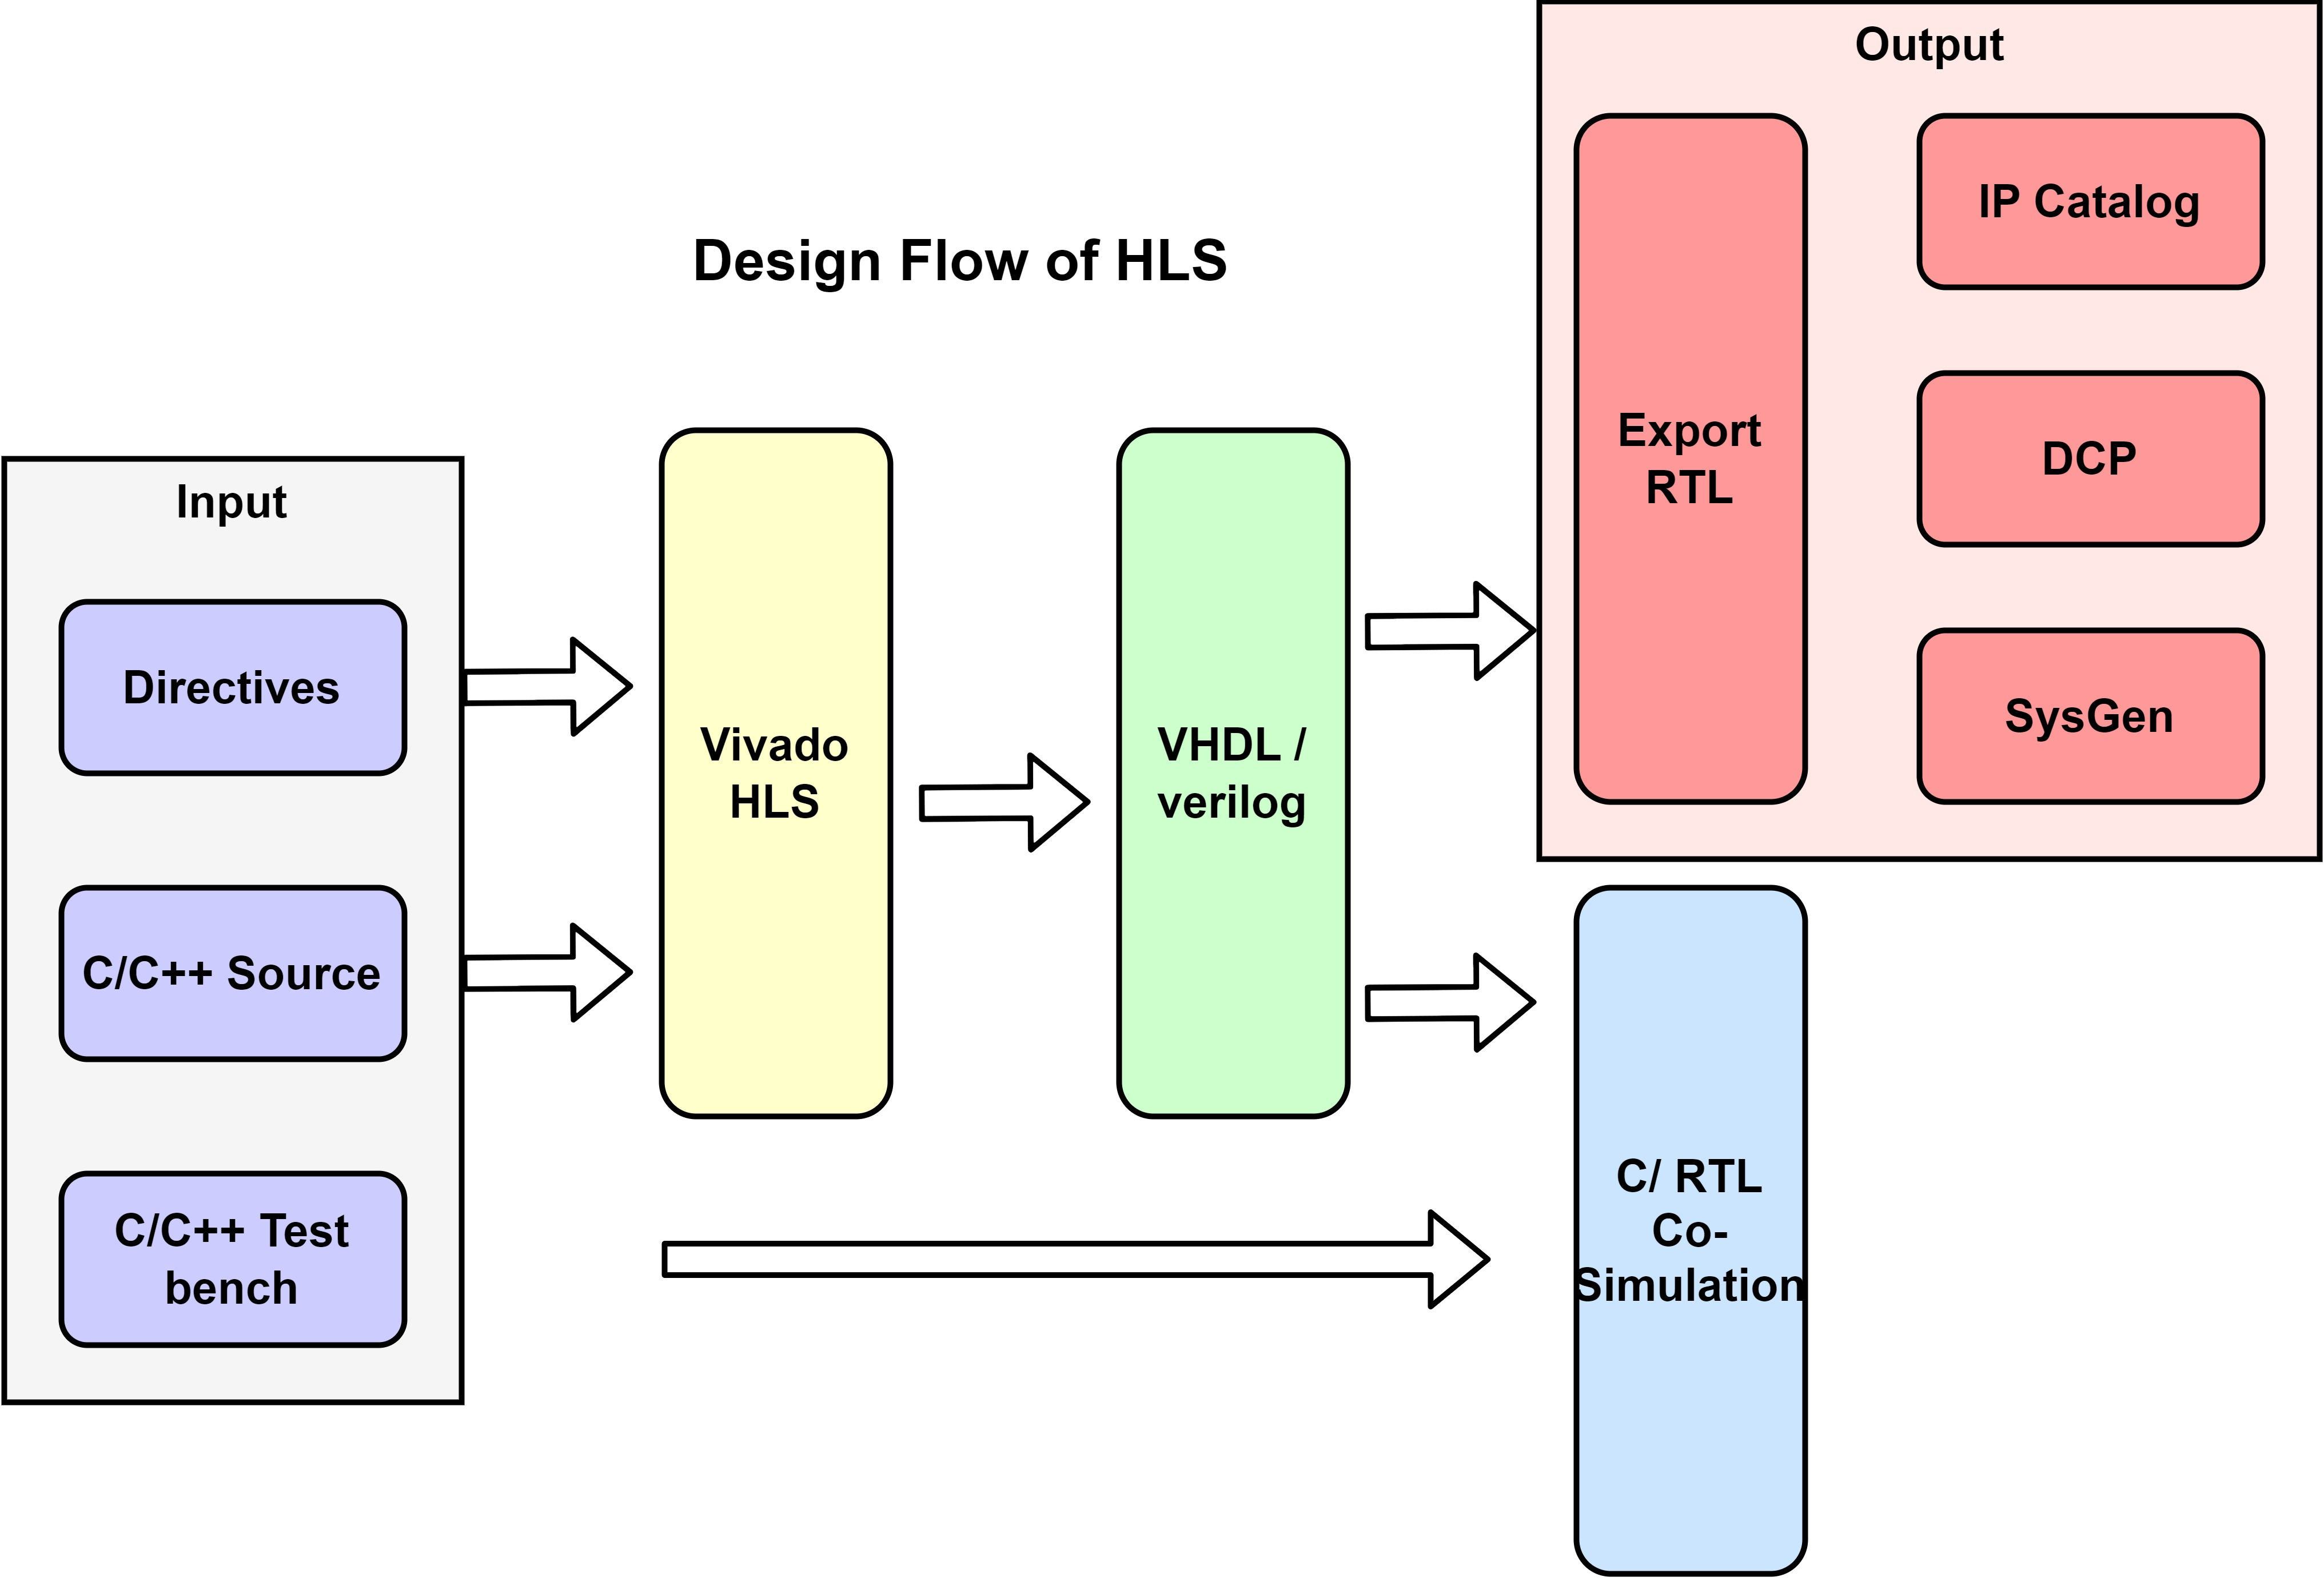
\includegraphics[width=0.8\textwidth]{Images/flow_LSI-Page-9.jpg}
    \caption{High-Level Synthesis design flow}
    \label{fig:hls_design_flow}
\end{figure}

The deployment flow in Figure~\ref{fig:hls_design_flow} consists of C/C++ design, functional simulation, synthesis, RTL export, Vivado integration, and board-level execution. During C/C++ simulation, the accelerator output is compared with the software reference to verify functional correctness. After synthesis, Vitis HLS reports latency estimates, initiation intervals, and resource usage, which are used to refine the architecture.

Several HLS techniques are applied in the implementation:
\begin{itemize}
    \item \textbf{Loop pipelining:} overlaps loop iterations so that new data can enter the datapath every cycle or after a short initiation interval.
    \item \textbf{Array partitioning:} increases memory bandwidth for frequently accessed buffers such as windows, weights, and partial sums.
    \item \textbf{Dataflow scheduling:} enables loading, computation, and output writing functions to execute concurrently.
    \item \textbf{Interface directives:} map large data arrays to AXI master ports and scalar control values to AXI4-Lite registers.
\end{itemize}

After the accelerator is exported as an IP core, Vivado is used to connect it with the Zynq Processing System, AXI interconnects, DDR memory, clocking, and reset logic. The final bitstream configures the PL with the generator accelerator. On the software side, a Vitis application running on the ARM processor prepares input buffers, writes configuration registers, launches the accelerator, and reads back the reconstructed image.

This implementation flow provides a complete path from neural network analysis to executable FPGA deployment. It also separates architectural design decisions in this chapter from the resource, timing, and performance evaluation reported in the following chapters.

%%%%%%%%%%%%%%%%%%%%%%%%%%%%%%%%%%%%%%%%%%%%%%%%%%%%%%%%%%%%%%%%%%%%%%%%%%%%%%%%%%%%%%%%%%%%%%%%%%%%
\subsection{Chapter Conclusion}

This chapter presented the implementation architecture of the HiFiC GAN accelerator. The system was organized as a hardware--software co-design in which the PS handles control and flexible processing, while the PL implements the complete generator -- the Fusion, UpConv, and Conv77 stages -- as a single accelerator IP.

The chapter also described the internal blocks, including line buffers, sliding windows, reflection padding, the processing element with its rotating accumulator, the two convolution and normalization/activation functional units, the three generator cores, the on-chip buffer layout, and the AXI kernel interface. Finally, the HLS and FPGA deployment flow was introduced to show how the C/C++ design is synthesized, integrated, and controlled on the ZCU104 platform. The next chapter evaluates the resulting FPGA implementation in terms of resource utilization, system integration, and performance.